\documentclass[14pt]{extbook}
\usepackage{multicol, enumerate, enumitem, hyperref, color, soul, setspace, parskip, fancyhdr} %General Packages
\usepackage{amssymb, amsthm, amsmath, latexsym, units, mathtools} %Math Packages
\everymath{\displaystyle} %All math in Display Style
% Packages with additional options
\usepackage[headsep=0.5cm,headheight=12pt, left=1 in,right= 1 in,top= 1 in,bottom= 1 in]{geometry}
\usepackage[usenames,dvipsnames]{xcolor}
\usepackage{dashrule}  % Package to use the command below to create lines between items
\newcommand{\litem}[1]{\item#1\hspace*{-1cm}\rule{\textwidth}{0.4pt}}
\pagestyle{fancy}
\lhead{Progress Quiz 2}
\chead{}
\rhead{Version C}
\lfoot{4389-3341}
\cfoot{}
\rfoot{Summer C 2021}
\begin{document}

\begin{enumerate}
\litem{
Solve the quadratic equation below. Then, choose the intervals that the solutions belong to, with $x_1 \leq x_2$ (if they exist).\[ -13x^{2} +9 x + 5 = 0 \]\begin{enumerate}[label=\Alph*.]
\item \( x_1 \in [-14.4, -11.6] \text{ and } x_2 \in [3.7, 6.6] \)
\item \( x_1 \in [-2.9, -0.7] \text{ and } x_2 \in [-0.8, 0.7] \)
\item \( x_1 \in [-0.9, 0.2] \text{ and } x_2 \in [0.9, 2.7] \)
\item \( x_1 \in [-18.2, -17.8] \text{ and } x_2 \in [16.8, 20.5] \)
\item \( \text{There are no Real solutions.} \)

\end{enumerate} }
\litem{
Factor the quadratic below. Then, choose the intervals that contain the constants in the form $(ax+b)(cx+d); b \leq d.$\[ 81x^{2} -81 x + 20 \]\begin{enumerate}[label=\Alph*.]
\item \( a \in [25.5, 30.5], \hspace*{5mm} b \in [-10, 0], \hspace*{5mm} c \in [2.3, 5], \text{ and } \hspace*{5mm} d \in [-8, -2] \)
\item \( a \in [8.6, 10.5], \hspace*{5mm} b \in [-10, 0], \hspace*{5mm} c \in [8.6, 10.9], \text{ and } \hspace*{5mm} d \in [-8, -2] \)
\item \( a \in [2.7, 4.5], \hspace*{5mm} b \in [-10, 0], \hspace*{5mm} c \in [26.3, 29.7], \text{ and } \hspace*{5mm} d \in [-8, -2] \)
\item \( a \in [0.7, 2.2], \hspace*{5mm} b \in [-51, -44], \hspace*{5mm} c \in [-2.6, 2.1], \text{ and } \hspace*{5mm} d \in [-38, -33] \)
\item \( \text{None of the above.} \)

\end{enumerate} }
\litem{
Graph the equation below.\[ f(x) = -(x+2)^2 - 16 \]\begin{enumerate}[label=\Alph*.]
\begin{multicols}{2}\item 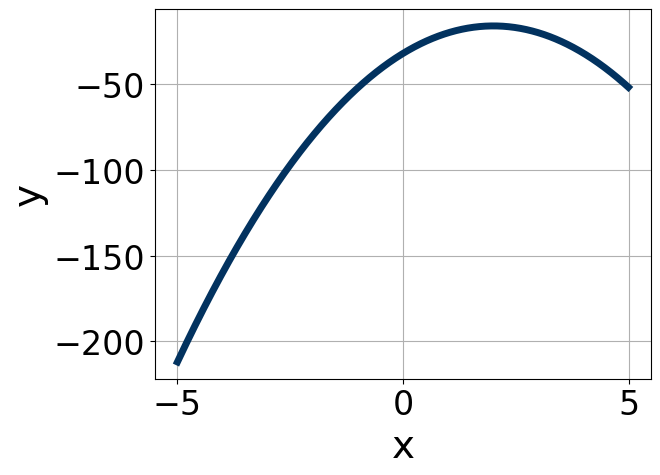
\includegraphics[width = 0.3\textwidth]{../Figures/quadraticEquationToGraphCopyAC.png}\item 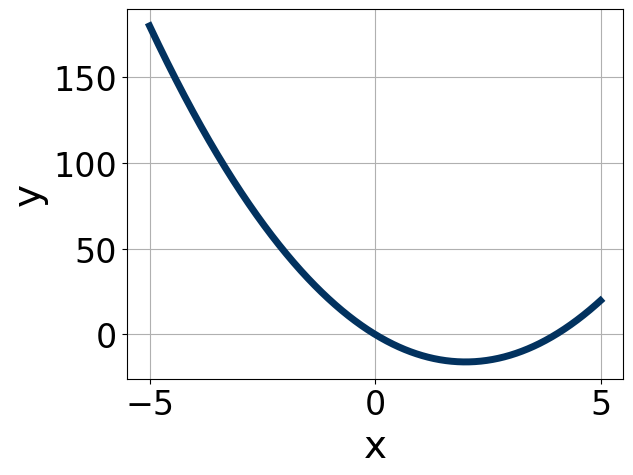
\includegraphics[width = 0.3\textwidth]{../Figures/quadraticEquationToGraphCopyBC.png}\item 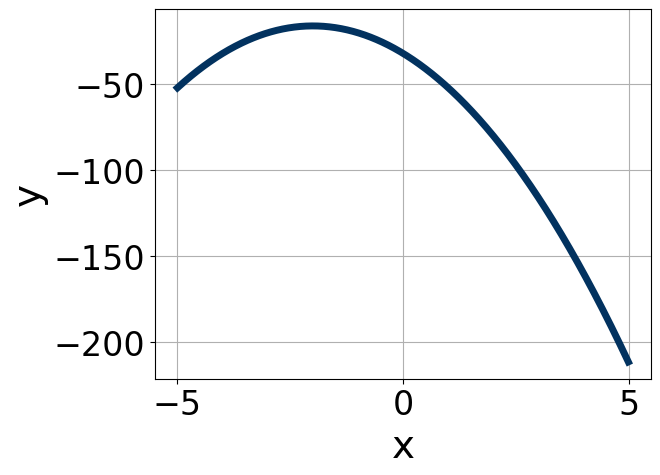
\includegraphics[width = 0.3\textwidth]{../Figures/quadraticEquationToGraphCopyCC.png}\item 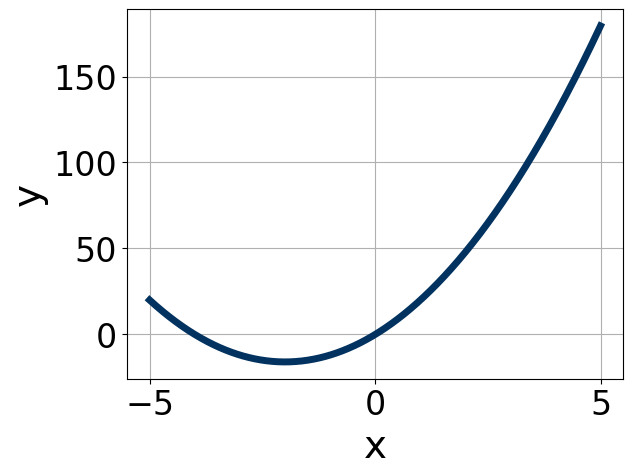
\includegraphics[width = 0.3\textwidth]{../Figures/quadraticEquationToGraphCopyDC.png}\end{multicols}\item None of the above.
\end{enumerate} }
\litem{
Graph the equation below.\[ f(x) = -(x+4)^2 - 19 \]\begin{enumerate}[label=\Alph*.]
\begin{multicols}{2}\item 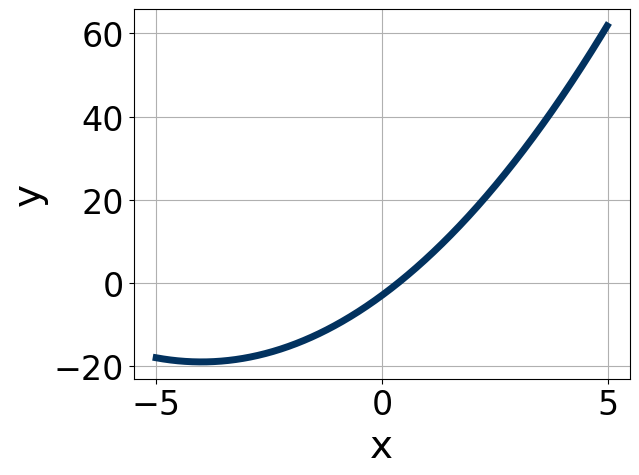
\includegraphics[width = 0.3\textwidth]{../Figures/quadraticEquationToGraphAC.png}\item 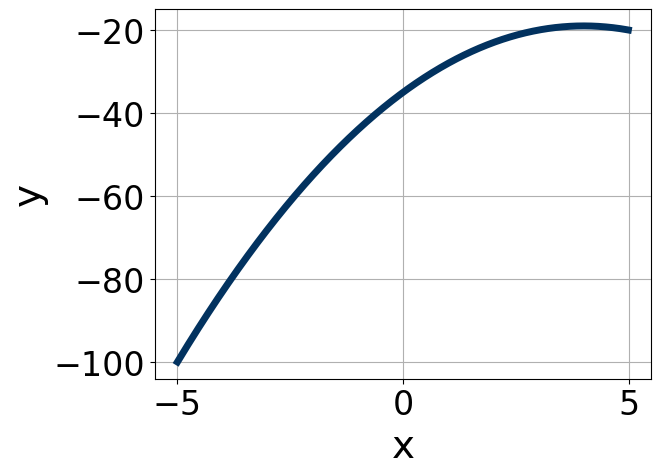
\includegraphics[width = 0.3\textwidth]{../Figures/quadraticEquationToGraphBC.png}\item 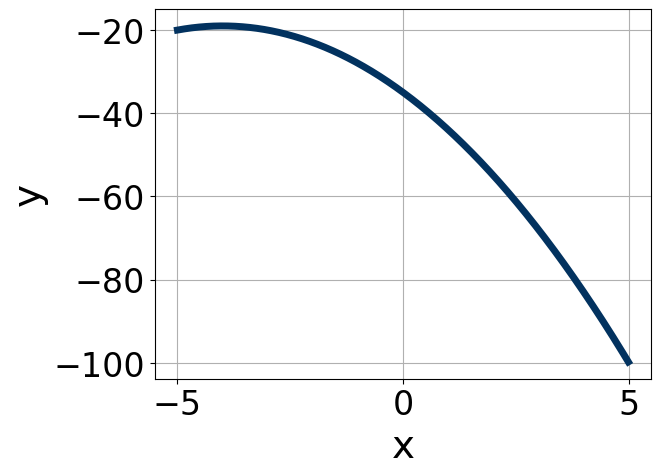
\includegraphics[width = 0.3\textwidth]{../Figures/quadraticEquationToGraphCC.png}\item 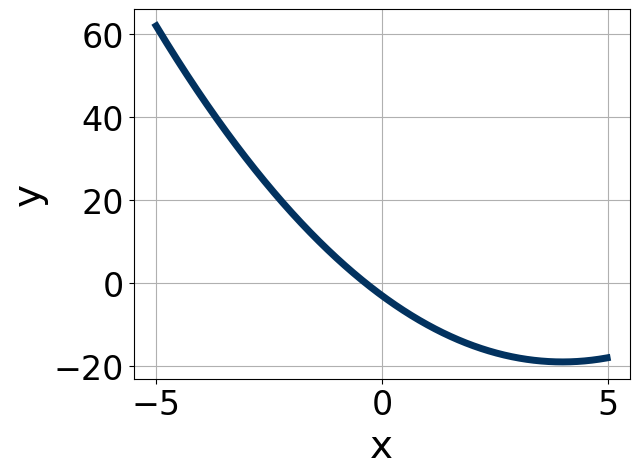
\includegraphics[width = 0.3\textwidth]{../Figures/quadraticEquationToGraphDC.png}\end{multicols}\item None of the above.
\end{enumerate} }
\litem{
Solve the quadratic equation below. Then, choose the intervals that the solutions belong to, with $x_1 \leq x_2$ (if they exist).\[ -14x^{2} -12 x + 7 = 0 \]\begin{enumerate}[label=\Alph*.]
\item \( x_1 \in [-6.23, -5.12] \text{ and } x_2 \in [16.63, 17.76] \)
\item \( x_1 \in [-1.75, -0.87] \text{ and } x_2 \in [0.18, 0.63] \)
\item \( x_1 \in [-24.6, -23.16] \text{ and } x_2 \in [22.45, 24.24] \)
\item \( x_1 \in [-0.6, 0.01] \text{ and } x_2 \in [1.13, 1.46] \)
\item \( \text{There are no Real solutions.} \)

\end{enumerate} }
\litem{
Write the equation of the graph presented below in the form $f(x)=ax^2+bx+c$, assuming  $a=1$ or $a=-1$. Then, choose the intervals that $a, b,$ and $c$ belong to.
\begin{center}
    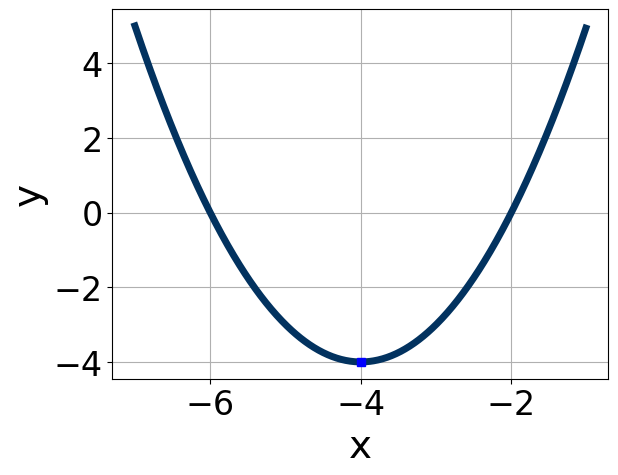
\includegraphics[width=0.5\textwidth]{../Figures/quadraticGraphToEquationC.png}
\end{center}
\begin{enumerate}[label=\Alph*.]
\item \( a \in [-1.1, 0.1], \hspace*{5mm} b \in [-12, -5], \text{ and } \hspace*{5mm} c \in [-22, -19] \)
\item \( a \in [0.5, 1.2], \hspace*{5mm} b \in [6, 9], \text{ and } \hspace*{5mm} c \in [9, 13] \)
\item \( a \in [-1.1, 0.1], \hspace*{5mm} b \in [6, 9], \text{ and } \hspace*{5mm} c \in [-22, -19] \)
\item \( a \in [0.5, 1.2], \hspace*{5mm} b \in [-12, -5], \text{ and } \hspace*{5mm} c \in [9, 13] \)
\item \( a \in [0.5, 1.2], \hspace*{5mm} b \in [-12, -5], \text{ and } \hspace*{5mm} c \in [20, 22] \)

\end{enumerate} }
\litem{
Solve the quadratic equation below. Then, choose the intervals that the solutions $x_1$ and $x_2$ belong to, with $x_1 \leq x_2$.\[ 15x^{2} +47 x + 36 = 0 \]\begin{enumerate}[label=\Alph*.]
\item \( x_1 \in [-13, -7.5] \text{ and } x_2 \in [-0.44, -0.12] \)
\item \( x_1 \in [-29.6, -26.2] \text{ and } x_2 \in [-20.19, -19.93] \)
\item \( x_1 \in [-2.2, 1.8] \text{ and } x_2 \in [-1.53, -1.1] \)
\item \( x_1 \in [-4.6, -2.5] \text{ and } x_2 \in [-1.03, -0.78] \)
\item \( x_1 \in [-7.8, -3.4] \text{ and } x_2 \in [-0.49, -0.4] \)

\end{enumerate} }
\litem{
Factor the quadratic below. Then, choose the intervals that contain the constants in the form $(ax+b)(cx+d); b \leq d.$\[ 36x^{2} +60 x + 25 \]\begin{enumerate}[label=\Alph*.]
\item \( a \in [10.5, 12.4], \hspace*{5mm} b \in [4, 7], \hspace*{5mm} c \in [2.19, 3.64], \text{ and } \hspace*{5mm} d \in [1, 7] \)
\item \( a \in [1.7, 5.9], \hspace*{5mm} b \in [4, 7], \hspace*{5mm} c \in [15.97, 19.02], \text{ and } \hspace*{5mm} d \in [1, 7] \)
\item \( a \in [0.9, 1.1], \hspace*{5mm} b \in [27, 35], \hspace*{5mm} c \in [0.58, 2.46], \text{ and } \hspace*{5mm} d \in [25, 33] \)
\item \( a \in [3.9, 6.8], \hspace*{5mm} b \in [4, 7], \hspace*{5mm} c \in [5.92, 6.33], \text{ and } \hspace*{5mm} d \in [1, 7] \)
\item \( \text{None of the above.} \)

\end{enumerate} }
\litem{
Write the equation of the graph presented below in the form $f(x)=ax^2+bx+c$, assuming  $a=1$ or $a=-1$. Then, choose the intervals that $a, b,$ and $c$ belong to.
\begin{center}
    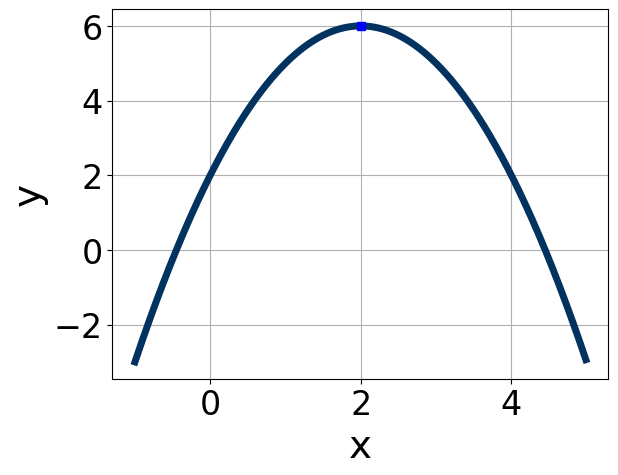
\includegraphics[width=0.5\textwidth]{../Figures/quadraticGraphToEquationCopyC.png}
\end{center}
\begin{enumerate}[label=\Alph*.]
\item \( a \in [0.8, 2.5], \hspace*{5mm} b \in [-4, -1], \text{ and } \hspace*{5mm} c \in [10, 13] \)
\item \( a \in [-1.3, -0.7], \hspace*{5mm} b \in [2, 6], \text{ and } \hspace*{5mm} c \in [0, 3] \)
\item \( a \in [0.8, 2.5], \hspace*{5mm} b \in [2, 6], \text{ and } \hspace*{5mm} c \in [10, 13] \)
\item \( a \in [-1.3, -0.7], \hspace*{5mm} b \in [-4, -1], \text{ and } \hspace*{5mm} c \in [0, 3] \)
\item \( a \in [-1.3, -0.7], \hspace*{5mm} b \in [-4, -1], \text{ and } \hspace*{5mm} c \in [-12, -8] \)

\end{enumerate} }
\litem{
Solve the quadratic equation below. Then, choose the intervals that the solutions $x_1$ and $x_2$ belong to, with $x_1 \leq x_2$.\[ 25x^{2} -15 x -54 = 0 \]\begin{enumerate}[label=\Alph*.]
\item \( x_1 \in [-6.39, -4.49] \text{ and } x_2 \in [0.33, 0.4] \)
\item \( x_1 \in [-30.32, -28.53] \text{ and } x_2 \in [44.96, 45.11] \)
\item \( x_1 \in [-0.41, 0.46] \text{ and } x_2 \in [5.38, 5.41] \)
\item \( x_1 \in [-1.92, -0.86] \text{ and } x_2 \in [1.7, 1.91] \)
\item \( x_1 \in [-4.03, -2.02] \text{ and } x_2 \in [0.49, 0.71] \)

\end{enumerate} }
\end{enumerate}

\end{document}